\subsection{Excercise DomainEntityCarV1.0}
\label{subsec:domain_entity_car_v1.0}
This task introduces the API design of the DM-Car.
It starts by taking a look at the used DDD pattern, and explaining why it is appropriate in this context.
After that, the used terms in the domain entity are described.
Finally, the example data is added to the table of example data, that can be found in the tasks sheet \cite{CM-T-DMC}.

\subsubsection*{DDD Pattern}
\label{subsubsec:ddd_pattern}
Domain-Driven-Design includes a set of patterns solving common problems elegantly.
These patterns are not necessarily new, yet they are grouped working in a new context.
Besides the already-known layered architecture pattern, the entity pattern is part of the DDD-core patterns.
An entity is described to be an object, that is not defined by its attributes, but by a thread of continuity and its identity.

A car is a good example of an entity because it is not defined by its attributes but by its identity.
In our case, the identity is the VIN (Vehicle Identification Number), the brand and the model.
The attributes can be the color, the engine, etc.
Even if the attributes change, the car is still the same entity due to its unique and therefore constant identity.
This concludes, the DDD pattern entity is an appropriate choice in this context.

\subsubsection*{Terms Used}
This section describes the terms used in the \texttt{domain\_entity\_car\_v1.0} file as it is shown in \texttt{gu\_terms\_used}.
\begin{table}[H]
    \centering
    \begin{tabular}{|p{5cm}|p{9cm}|}
        \hline
        \textbf{Term} & \textbf{Definition} \\
        \hline
        Domain Entity & This shows, that this entity is part of the domain. \\
        Car & \texttt{Car} is part of the domain. 
        It represents a car that can be used application-agnostically in various applications related to the domain. \\
        \hline
        Vin & The VIN (Vehicle Identification Number) is a unique identifier for a car.\\
        \hline
        Brand & This is the name of the car's brand.\\
        \hline
        Model & This is the name of the car's model.\\
        \hline
    \end{tabular}
    \caption{Terms Used in DomainEntityCarV1.0}
    \label{tab:terms_used_domain_entity_car_v1.0}
\end{table}

\subsubsection*{Example Data}
This task adds the example data to the table of example data.
The example data is given in the task sheet.
The results are shown in \autoref{tab:example_data_domain_entity_car_v1.0}.
\begin{table}[H]
    \centering
    \begin{tabular}{|p{5cm}|p{2cm}|p{2cm}|}
        \hline
        vin & brand & model \\
        \hline
        JH4DB1561NS000565 & VW & ID2 \\
        JN8AZ2NC5B9300256 & VW & ID3 \\
        2FDKF38G3KCA42390 & Ford & Mustang \\
        1GBJK39DX6E165432 & Tesla & Model S \\
        JH4DB1550MS003978 & Audi & A3 \\
        \hline
    \end{tabular}
    \caption{Example Data of DomainEntityCarV1.0}
    \label{tab:example_data_domain_entity_car_v1.0}
\end{table}

\subsection{Excercise APIDiagramDMCarV1.0}
\label{subsec:api_diagram_dm_car_v1.0}
This task takes a closer look at the API diagram of the DM-Car.
First, the relationship between the collection and the domain entity is described.
An alternative is provided and the pros and cons of both are discussed.
After that, the different API styles ReST and gRPC are introduced.
It is discussed which one is more appropriate in this context.
\subsubsection*{Relationship Between Cars and Car}
% Description of the Relationship
The \texttt{api\_diagram\_dm-car\_v1.0} file in the \texttt{pages} folder describes the relationship between the collection \texttt{cars} and the domain entity \texttt{car}.
It provides a clear overview of the domain microservice \texttt{DM-CarV1.0}.

As mentioned, \texttt{Cars} is a collection of \texttt{Car}.
It therefore contains a list of \texttt{Car} objects.
Furthermore, the collection of cars provides the methods used in each car entity.
"\texttt{getCar(vin: Vin): Car}" takes a VIN and returns the car with the given VIN.
"\texttt{getCars(): Car[]}" takes no parameters and returns the list of all cars held by the collection.

This is a 1-to-many relationship, with the collection being the 1 and the car being the n.
N can be zero.
Therefore the collection is unique and can be empty.

% Providing an alternative and discussing the pros and cons of both
The alternative modeling of the relationship is shown in \autoref{fig:api_diagram_dm_car_alternative}.

It also uses the collection of cars and the car entity.
Yet, instead of providing the methods in the collection, the methods are provided by using the factory software pattern.
The factory \texttt{CarFactory} implements the \texttt{ICarFactory} interface.
The factory provides the methods "\texttt{getCar(vin: Vin): Car}" that were provided by the collection in the first model.
Therefore the collection is only used to store the cars.
This provides a better separation of concerns by separating the storage and the logic.
Yet, the relationship between the collection and the car is not as clear as in the first model.
However, the second model is more flexible.
It is easier to change the storage of the cars without changing the logic.

Therefore both models have their pros and cons.

\begin{figure}[H]
    \centering
    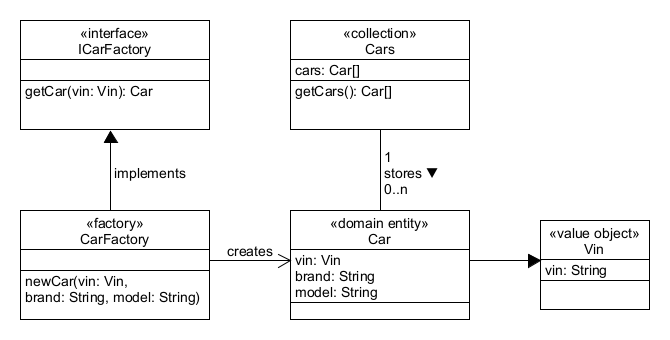
\includegraphics[width=0.8\textwidth]{figures/microservices/dmCar/apiDiagramDM-CarExtended.png}
    \caption{Alternative API Diagram of DM-CarV1.0}
    \label{fig:api_diagram_dm_car_alternative}
\end{figure}

\subsubsection*{API Operations}
As mentioned in \autoref{subsec:rest_and_grpc} gRPC and ReST are two different approaches to implementing an API.
Their main difference is their orientation in the way they communicate.
While gRPC is method-oriented, ReST is resource-oriented.

\texttt{DM-CarV1.0} is a domain-microservice implementing CRUD operations on car entities.
Therefore, the main focus of the microservice is resource-oriented.
This makes ReST the better choice for this microservice.

\subsection{Excercise PrepareLocalWorkingFolder}
\label{subsec:prepare_local_working_folder}
After cloning the repository \texttt{DM-Car} of the \texttt{3.MicroserviceEngineering} an analysis of the repository is done.
The following section describes the relations to the architectural diagram from the previous exercise 

\paragraph*{General Folder Structure:}
Opening the root folder of the repository, three folders and a \texttt{README.md} file is found.
The \texttt{README.md} file contains a short description of how to set up the database and run the domain microservice.
\texttt{pages} contains the API diagram of the microservice.
The \texttt{figures} folder contains the figures used in the API diagram. 
The \texttt{src} folder contains the source code of the microservice that will be further analyzed in the following paragraph.

\paragraph*{src:}
Opening the folder, the structure shown in \autoref{fig:ms_dmCar_srcFolderStructure} is found.

\texttt{go.mod} contains the dependencies of the microservice, linking to the used repositories and their versions.
\texttt{go.sum} contains the checksums of these dependencies, acting as a security measure.
\texttt{main.go} is the main file of the microservice creating the Postgres database and starting the server.
This file is compiled into an executable file.

\paragraph*{Relations to the Architectural Diagram:}
The architectural diagram of the microservice is modeled in the repository, implementing the entities and the according functions.
Therefore, this repository contains the implementation of the domain microservice \texttt{DM-CarV1.0} inside the domain logic layer of the application.

The collection \texttt{Cars} and the domain entity \texttt{Car} are implemented in the \texttt{Cars.go} and \texttt{Car.go} files respectively.
Both files can be found in the \texttt{/src/logic/model} folder.
Both files implement the attributes of the entities, yet they do not implement the methods shown in the diagram.

The methods are implemented separately with each method having its file.
According files are found in the \texttt{/src/logic/operations} folder.
Therefore, it is not possible to identify which method belongs to which entity.

The value object \texttt{Vin} used by \texttt{Car} is implemented in the \texttt{Vin.go} file.
The file also can be found in the \texttt{/src/logic/model} folder.
It implements the "\texttt{IsValidVin()}" method checking if a VIN is valid, yet this is not shown in the diagram.

Also, further functionalities like mappers, handlers, etc. are not shown in the diagram.
However, they are essential for the microservice to work.
They are implemented in the \texttt{/src/infrastructure} and \texttt{/src/api} folders.

To conclude, general relations between the implementation and the diagram are met.
\texttt{Cars} is a collection of \texttt{Car} and all entities are implemented as shown in the diagram.
Yet, methods are not implemented in the entities but in separate files.
Furthermore, the value object \texttt{Vin} implements further functions not shown in the diagram.
Also, further functionalities like mappers, handlers, etc. are not shown in the diagram.

\begin{figure}
    \centering
    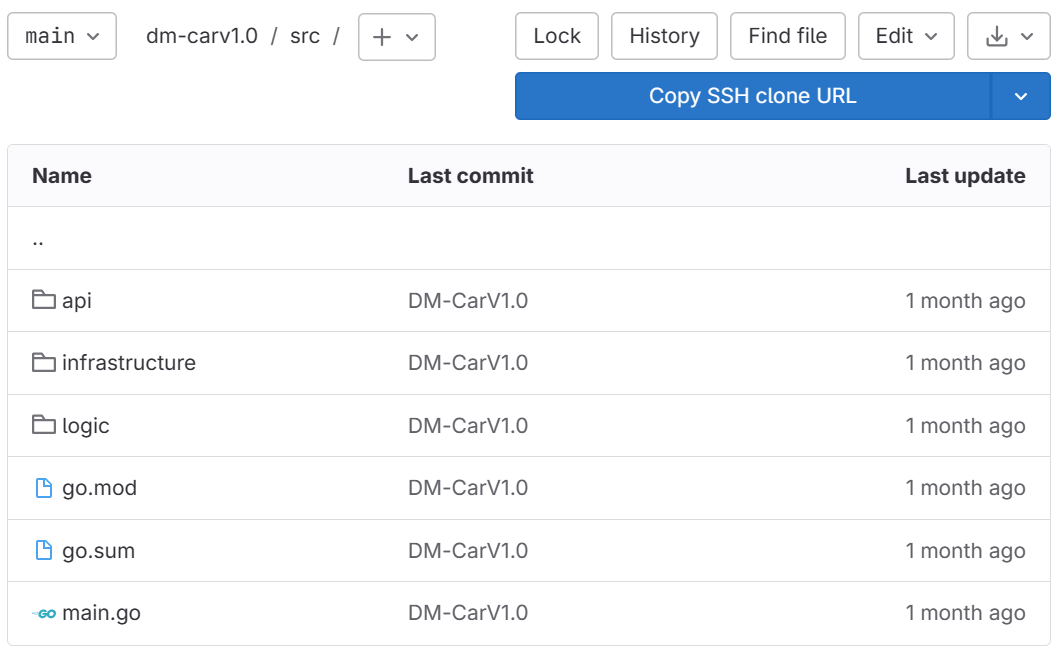
\includegraphics[width=0.8\textwidth]{figures/microservices/dmCar/ms_dmCar_srcFolderStructure.png}
    \caption{Folder Structure of the src Folder}
    \label{fig:ms_dmCar_srcFolderStructure}
\end{figure}
